%!TEX TS-program = lualatex
%!TEX encoding = UTF-8 Unicode

\documentclass[12pt, hidelinks]{exam}
\usepackage{graphicx}
	\graphicspath{{/Users/goby/Pictures/teach/163/lab/}
	{img/}} % set of paths to search for images

\usepackage{geometry}
\geometry{letterpaper, left=1.5in, bottom=1in}                   
%\geometry{landscape}                % Activate for for rotated page geometry
\usepackage[parfill]{parskip}    % Activate to begin paragraphs with an empty line rather than an indent
\usepackage{amssymb, amsmath}
\usepackage{mathtools}
	\everymath{\displaystyle}

\usepackage{fontspec}
\setmainfont[Ligatures={TeX}, BoldFont={* Bold}, ItalicFont={* Italic}, BoldItalicFont={* BoldItalic}, Numbers={OldStyle}]{Linux Libertine O}
\setsansfont[Scale=MatchLowercase,Ligatures=TeX, Numbers=OldStyle]{Linux Biolinum O}
%\setmonofont[Scale=MatchLowercase]{Inconsolatazi4}
\usepackage{microtype}


% To define fonts for particular uses within a document. For example, 
% This sets the Libertine font to use tabular number format for tables.
 %\newfontfamily{\tablenumbers}[Numbers={Monospaced}]{Linux Libertine O}
% \newfontfamily{\libertinedisplay}{Linux Libertine Display O}

\usepackage{booktabs}
\usepackage{multicol}

\usepackage{tikz}
\usepackage{forest}
\forestset{
    every leaf node/.style={
        if n children=0{#1}{}
    },
    every tree node/.style={
        if n children=0{}{#1}
    },
    mytree/.style={
        for tree={
            edge path={
            \noexpand\path [draw, very thick, \forestoption{edge}] (!u.parent anchor) |- (.child anchor)\forestoption{edge label};
            },
            every tree node={draw=none,inner sep=0, outer sep=0, minimum size=0},
            every leaf node/.style={align=left},
            grow=east,
            parent anchor=south, 
            child anchor=west,
            anchor=west,
            l sep=5mm,
            s sep=3mm,
            draw=none,
    			if n children=0{tier=word}{}
        }
    }
}



\usepackage{longtable}
%\usepackage{siunitx}
\usepackage{array}
\newcolumntype{L}[1]{>{\raggedright\let\newline\\\arraybackslash\hspace{0pt}}p{#1}}
\newcolumntype{C}[1]{>{\centering\let\newline\\\arraybackslash\hspace{0pt}}p{#1}}
\newcolumntype{R}[1]{>{\raggedleft\let\newline\\\arraybackslash\hspace{0pt}}p{#1}}

\usepackage{enumitem}
\setlist{leftmargin=*}
\setlist[1]{labelindent=\parindent}
\setlist[enumerate]{label=\textsc{\alph*}.}
\setlist[itemize]{label=\color{gray}\textbullet}

\usepackage{hyperref}
%\usepackage{hanging}

\usepackage[sc]{titlesec}

%% Commands for Exam class
\renewcommand{\solutiontitle}{\noindent}
\unframedsolutions
\SolutionEmphasis{\bfseries}

\renewcommand{\questionshook}{%
	\setlength{\leftmargin}{-\leftskip}%
}

\newcommand{\hidepoints}{%
	\pointsinmargin\pointformat{}
}

\newcommand{\showpoints}{%
	\nopointsinmargin\pointformat{(\thepoints)}
}

\pagestyle{headandfoot}
\firstpageheader{\textsc{bi}\,063 Evolution and Ecology}{}{\ifprintanswers\textbf{KEY}\else Name: \enspace \makebox[2.5in]{\hrulefill}\fi}
\runningheader{}{}{\footnotesize{pg. \thepage}}
\footer{}{}{}
\runningheadrule

\newcommand*\AnswerBox[2]{%
    \parbox[t][#1]{0.92\textwidth}{%
    \begin{solution}#2\end{solution}}
    \vspace{\stretch{1}}
}

\newenvironment{AnswerPage}[1]
    {\begin{minipage}[t][#1]{0.92\textwidth}%
    \begin{solution}}
    {\end{solution}\end{minipage}
    \vspace{\stretch{1}}}

\newlength{\basespace}
\setlength{\basespace}{5\baselineskip}


%
%\makeatletter
%\def\SetTotalwidth{\advance\linewidth by \@totalleftmargin
%\@totalleftmargin=0pt}
%\makeatother

\usepackage{wrapfig}

%\printanswers

\newlength{\tempintextsep}
\setlength{\tempintextsep}{\intextsep}

\begin{document}

\subsection*{Transitional forms and the fossil record}% (\numpoints\ points)}


\setlength{\intextsep}{0pt}

%\begin{center}
\begin{wrapfigure}[10]{r}[23pt]{0pt}
\begin{forest} mytree
[[	
	[cat]
	[fish]
	[human]
	[pigeon]
	[turtle]
	[salamander]
]]
\end{forest}
%	\begin{tikzpicture}
%		[branch/.style={thick}]
%		
%		\draw [branch] (0,0) -- (0,1);
%		\draw [branch] (0,1) -- (-3,4) node [above] {\strut cat};
%		\draw [branch] (0,1) -- (-2,4) node [above] {\strut fish};
%		\draw [branch] (0,1) -- (-0.75,4) node [above] {\strut human};
%		\draw [branch] (0,1) -- (0.75,4) node [above] {\strut pigeon};
%		\draw [branch] (0,1) -- (2,4) node [above] {\strut turtle};
%		\draw [branch] (0,1) -- (3,4) node [above right, xshift=-10pt] {\strut salamder};
%
%	\end{tikzpicture}
\end{wrapfigure} After the examining the skeletal evidence, you should have a 
tree that looks similar to the one shown at right. The skeletons and embryos
provided evidence of common ancestry for the six organisms but not enough to resolve 
the the relationships of each one. Other skeletal evidence exists
that can resolve relationships, but it is hard to use in a course like this.
 Instead, you will use evidence from the fossil record. % \bigskip

%\end{center}



\setlength{\intextsep}{\tempintextsep}

\begin{wrapfigure}[13]{r}{0pt}
%	\includegraphics[width=0.45\textwidth]{07_transitional_tree_full}
	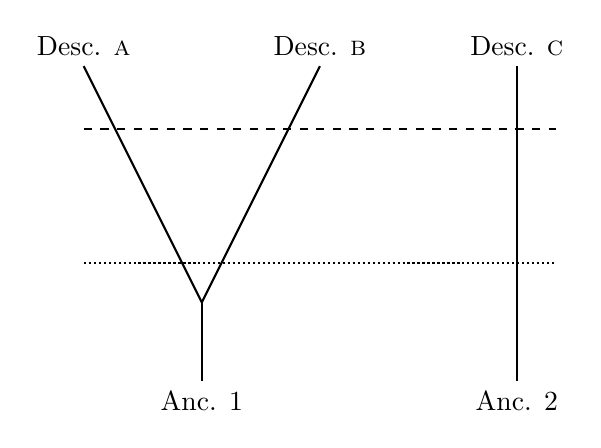
\begin{tikzpicture}
		[branch/.style={thick}]
		\draw [branch] (-1.5,0) node [below] {Anc. 1} -- (-1.5,1);
		\draw [branch] (-1.5,1) -- (-3,4) node [above] {Desc. \textsc{a}};
		\draw [branch] (-1.5,1) -- (0,4) node [above] {Desc. \textsc{b}};
		\draw [branch] (2.5,0) node [below] {Anc. 2} -- (2.5,4) node [above] {Desc. \textsc{c}};
		
		\draw [densely dotted, thick] (-3,1.5) -- (3,1.5);
		\draw [dashed, thick] (-3,3.2) -- (3,3.2);
		
	\end{tikzpicture}
\end{wrapfigure}Fossils provide evidence of common ancestry because of descent with modification, meaning that species share an ancestor but some of their traits have been modified from the ancestral form. Modified traits do not appear suddenly but slowly become different over time, shown in the tree at right. Descendants \textsc{a} and \textsc{b} are predicted to share Ancestor~1. Soon after speciation (dotted line), the descendants still strongly resemble the ancestor but some traits will be slightly modified. Much later (dashed line), the descendants look less like their ancestor and more like their final forms. 

The fossils that show these changing traits are called \textit{transitional forms.} A transitional form is an intermediate species found in the fossil record that contains traits of both the ancestor and the descendant. Transitional forms should appear only between organisms that do have a common ancestor.  In the tree above, transitional forms should appear between Ancestor~1 and Descendants~\textsc{a} and \textsc{b}. Transitional forms should \textit{not} appear Ancestor~1 and Descendant~\textsc{c}.  If a transitional form were found between Ancestor~1 and Descendant~\textsc{c}, then the hypothesis would be falsified. Similarly, if a transitional form were found between Ancestor~2 and Descendants~\textsc{a} or \textsc{b}, then the hypothesis would be falsified.

\begin{questions}

\question
Study the two phylogenetic trees (hypotheses) on the next page.  Think carefully about the type of transitional fossils that are \emph{predicted} by \textit{each} hypothesis. Then, answer the questions after the trees.

\newpage

Hypothesis 1:

\begin{center}

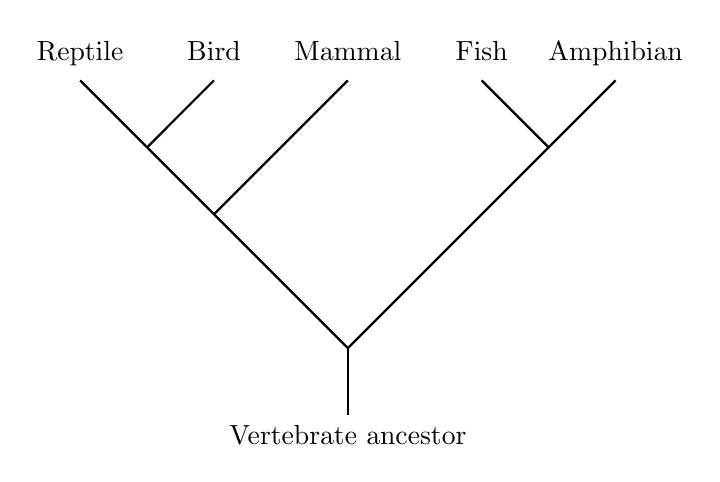
\begin{tikzpicture}
	[scale=0.85, branch/.style={thick}]
	
	\coordinate (root) at (0,0);
	\coordinate (rm) at (-2,2);
	\coordinate (rb) at (-3,3);
	\coordinate (fa) at (3,3);
	\draw [branch] (0,-1) node [below] {Vertebrate ancestor} -- (root);
	\draw [branch] (root) -- (rm);
	\draw [branch] (rm) -- (-0,4) node [above] {\strut Mammal}; % mammals
	\draw [branch] (rm) -- (rb);
	\draw [branch] (rb) -- (-2,4) node [above] {\strut Bird}; % birds
	\draw [branch] (rb) -- (-4,4) node [above] {\strut Reptile}; %reptiles
	\draw [branch] (root) -- (fa);
	\draw [branch] (fa) -- (4,4) node [above] {\strut Amphibian};
	\draw [branch] (fa) -- (2,4) node [above] {\strut Fish};
	
\end{tikzpicture}\label{hypothesis1}

\end{center}

\bigskip

Hypothesis 2:

\begin{center}

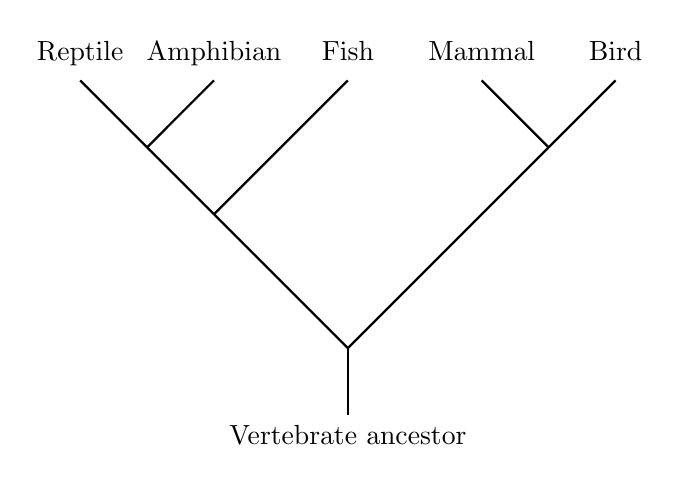
\begin{tikzpicture}
	[scale=0.85,branch/.style={thick}]
	
	\coordinate (root) at (0,0);
	\coordinate (rm) at (-2,2);
	\coordinate (rb) at (-3,3);
	\coordinate (fa) at (3,3);
	\draw [branch] (0,-1) node [below] {Vertebrate ancestor} -- (root);
	\draw [branch] (root) -- (rm);
	\draw [branch] (rm) -- (-0,4) node [above] {\strut Fish}; % mammals
	\draw [branch] (rm) -- (rb);
	\draw [branch] (rb) -- (-2,4) node [above] {\strut Amphibian}; % birds
	\draw [branch] (rb) -- (-4,4) node [above] {\strut Reptile}; %reptiles
	\draw [branch] (root) -- (fa);
	\draw [branch] (fa) -- (4,4) node [above] {\strut Bird};
	\draw [branch] (fa) -- (2,4) node [above] {\strut Mammal};
	
\end{tikzpicture}\label{hypothesis2}

\end{center}

\bigskip

\begin{parts}

	\part Which tree(s) predict a transition between reptiles and mammals? \ifprintanswers\textbf{A}\fi

	\vspace{\stretch{1}}

	\part Which tree(s) predict a transition between reptiles and birds?  \ifprintanswers\textbf{A}\fi
	
	\vspace{\stretch{1}}
	
	\part Which tree(s) predict a transition between birds and mammals?   \ifprintanswers\textbf{B}\fi

	\vspace{\stretch{1}}
	
	\part Which tree(s) predict a transition between fishes and amphibians?  \ifprintanswers\textbf{A and B}\fi
	
	\vspace{\stretch{1}}
	
	\part Which tree(s) predict a transition between amphibians and reptiles?  \ifprintanswers\textbf{B and arguably A}\fi

	
\end{parts}

\newpage

\subsubsection*{Reptile / mammal transition: predictions}

Mammals are distinguished from reptiles by many traits, like being warm-blooded, giving live birth, and having mammary glands. These traits, however, do not appear in fossil mammals. Fortunately, mammals and reptiles have different features in their skulls that allow you to easily tell whether a fossil was a mammal or a reptile.  Zoologists distinguish between reptiles and mammals primarily by the structure of the lower jaw.  Most reptiles, along with birds and amphibians, have skulls that look roughly like this:

\begin{center}\includegraphics[width=0.7\textwidth]{07_reptile_skull}\end{center}

Turtles and crocodilians (alligators, etc.) have some differences from this model, but the jaw structure is essentially the same in them, too.  Note that each side of the lower jaw in these organisms is composed of several bones:  the dentary, which carries the teeth (hence the name), somewhere between 2 and 5 other bones, and the articular, which actually makes contact with the skull (articulates with it) to form the jaw joint (hence its name).  The bone in the skull that makes contact with the articular is the quadrate.  Therefore, reptiles, birds, and amphibians have a \emph{quadrate-articular} jaw joint.  

Now look at a mammalian skull:

	\begin{center}\includegraphics[width=0.7\textwidth]{07_mammal_skull} \end{center}
	
Note that the dentary is the only bone in the lower jaw of a mammal—one on each side.  The dentary makes contact with a bone in the skull called the squamosal, forming a \emph{dentary-squamosal} jaw joint. 

There are some other bone differences between reptiles and mammals.  Reptiles mostly have no separation between the nasal passages and the mouth.  In mammals, they are separated by a plate of bone called the secondary palate.  Reptiles have teeth that are all simple cones, each with a single root.  Mammals have teeth of a variety of types, some of which have multiple points, or cusps, and multiple roots.  

Look again at the two hypotheses above (page~\pageref{hypothesis1}). Hypothesis~1 predicts that reptiles and mammals have a common ancestor and so should have transitional forms. Hypothesis~2 does not make this prediction. Now, reptiles are found in the fossil record starting in rocks dating to about 320 million years ago, while the earliest mammal fossils are in rocks dating to about 220 million years ago.\footnote{The techniques by which fossils are dated will be briefly covered in lecture. The dates provided here are the generally accepted dates for various fossils and rock formations, independently confirmed by lots of labs, with a margin of error well under 5\%.  (Ideas and illustrations in this page based on Hopson, JA 1987.  The Mammal-Like Reptiles.  American Biology Teacher 49:16-26)}  So, hypothesis 1 predicts that mammals evolved from some early reptile (rather than the other way around). Hypothesis~1 would therefore predict that we should see a series of organisms in the past that get gradually more and more like mammals and less like reptiles (of course, other reptiles continue being reptiles and get more similar to modern reptiles over time).  

\question
Specifically, in terms of jaw, tooth, and type of jaw joint identified above, what does hypothesis~1 predict you should see in these extinct transitional fossils?  Explain.

\AnswerBox{6\baselineskip}{%
Hypothesis 1 predicts that the dentary bone should enlarge to become the entire lower jaw, the teeth should change from conical to complex, rooted teeth, and the articular-quadrate joint should get replaced by the dentary-squamosal joint; 
}


\question
Hypothesis 2, on the other hand, predicts that you should not see a gradual progression from reptile to more and more mammalian, but rather that you will see extinct reptiles and extinct mammals.  Any ``in between'' characteristics will just be chance resemblances.  So, in terms of jaw, tooth,  and type of jaw joint, what does hypothesis~2 predict we'll see in extinct organisms?  Explain.

\AnswerBox{6\baselineskip}{%
Hypothesis 2 predictions that none of the features should change. Reptile skulls should have multiple bones in the lower jaw, the teeth should always be conical, and they should always have an articular-quadrate bone. Mammal skulls should always have only a dentary bone for the lower jaw, complex rooted teeth, and a dentary-squamosal joint.}

\newpage

\subsubsection*{Reptile / mammal transition: fossil evidence}

Hypothesis~1 predicts that you should see successive stages from ``very reptilian'' to
``very mammalian.'' Here are three ways to tell reptiles from mammals by their bones:

%predicting not just that there will be found some remains of organisms
%that are sort of in between reptiles and mammals, but that you should see
%successive stages in this process, going from ``very reptilian'' to
%``very mammalian.''

%There were four main ways to tell reptiles from mammals by their bones:

\begin{itemize}
\item
  jaws (multiple bones in lower jaw, vs only dentary)
\item
  jaw joint (quadrate-articular vs dentary-squamosal)
\item
  teeth (simple cones vs varied, with multiple cusps and roots)
%\item
%  secondary palate (absent vs present)
\end{itemize}

%The first two both have to do with jaws so look first at the jaws of
%some extinct animals. Diagrams of the skulls of eight different fossil species are at your
%desk. 
Your instructor will handout diagrams of the skulls of eight fossil species.
Here are what the abbreviations on the diagrams stand for:

\begin{longtable}[c]{@{}L{0.22\textwidth}L{0.22\textwidth}L{0.22\textwidth}L{0.22\textwidth}@{}}
\toprule
a - angular & dent - dentary & part - prearticular & qj -
quadratojugal\tabularnewline
\midrule
\endhead
ang - angular & j - jugal & pf - prefrontal & ref lam - reflected lamina
of angular\tabularnewline
art - articular & max - maxilla & po - postorbital & sa -
surangular\tabularnewline
d - dentary & pal - palatine & q - quadrate & sq -
squamosal\tabularnewline
& & & sur - surangular\tabularnewline
\bottomrule
\end{longtable}

In each diagram, the dentary has been highlighted. Since the dentary is the whole jaw in mammals, but a relatively
small part of the jaw in reptiles, you should be able to arrange these
in order from most reptilian to most mammalian based on the proportion
of the lower jaw that is the dentary. Arrange the skull pictures from most reptilian to most mammalian based on the
size of the dentary in the lower jaw, relative to the size of the entire
lower jaw, the type of jaw joint, and the type of teeth.

\question \label{order_question}
Write the names in your order of most reptile-like to most mammal-like.

\AnswerBox{2\baselineskip}{Approx: Sphenacodontid, Biarmosuchian,
Theriodont, \textit{Procynosuchus, Thrinaxodon, Probainognathus, Ictidosaur,} and \textit{Morganucodon.}}

%With your animals arranged from most reptilian to most mammalian based
%only on the dentary, look at the teeth.
%
%\question
%Do you notice any distinctive transitional pattern between
%reptilian-like teeth and mammalian-like teeth? Explain.
%
%\AnswerBox{2\baselineskip}{%
%General trend from conical reptilian to differentiated mammal-like.
%}
%
%\question
%Describe the trend that you observe for the dentary bone.
%
\question
Based on your results, what can you conclude about Hypothesis~1 and Hypothesis~2 from page~\pageref{hypothesis1}? Explain.

\AnswerBox{2\baselineskip}{%
Hypothesis~1 predicted transitional forms between reptiles and mammals. Transitional forms were found so H1 was supported. %Because hypothesis 2 predicted no common ancestor between reptiles and mammals, H2 was falsified.
}

So far, you have arranged these fossils in order according to how reptilian or mammalian they appear.  The fossils themselves were found in rock formations of various ages, and those rock formations can be dated, in most cases within a range of about 5\% of the total age.  Thus there is a natural sequence for when these organisms lived.  You could put them in order based on the age of the rocks you find their fossils in, from oldest to youngest rocks to see the order in which they appear in the fossil record. 

\question
If hypothesis~1 is right, mammals evolved from reptile ancestors.  What does hypothesis~1 predict you should you see if you arrange these organisms in order based on the age of the rocks in which their fossils are found?  Explain.

\AnswerBox{4\baselineskip}{%
	Predicts that the order of the organisms listed in question~\ref{order_question} is the order they should appear in the fossil record. The first listed above should appear first in the fossil record (be the oldest). The last is the list should appear last in the fossil record (be the youngest). 
}

%\question
%If hypothesis 2 is right, mammals, reptiles, and these ``mammal-like reptiles'' are unrelated, and any similarities are due to analogy.   What does hypothesis~2 predict about the order of appearance of these fossil organisms in the fossil record? Explain. 
%
%\AnswerBox{1\baselineskip}{The order should be random.}
%\newpage
%
Below is a diagram showing the ages of rocks in which the various
fossils were found. The numbers across the top are millions of
years before the present. There are some organisms included here that you
have not seen because pictures of their complete skulls were not available 
but the skull features are consistent with your results.

\begin{center}
\includegraphics[width=0.95\textwidth]{07_fossil_appearance}
\end{center}

Compare the jaw sequences with the time of appearance in the
fossil record. Some of these groups of organisms were around apparently
only a fairly short time, while other groups lasted much longer. It is possible
that some of the organisms lived for longer periods but fossils have not yet been
found outside the times shown. Therefore the order of the groups of organisms in the diagram is based on earliest
appearance in the fossil record, to represent the time when that
group first arose. Note also that \textit{Morganucodon} is included
in ``mammals,'' as the earliest known
fossil mammal.

These groups represent different taxonomic levels, also. Some of the
groups above are genus names (\emph{Probainognathus, Morganucodon,
Thrinaxodon}), while others are families or even larger groups like a class 
(mammals). This is one reason why some groups did not last as
long. A single genus might become extinct, while other genera in the
same family might survive. Do not worry about the taxonomic
levels; the information is included for clarity.

\question
What do you conclude about hypothesis~1 based on the
evidence from time of appearance in the fossil record of the various
mammal-like reptiles? Explain. 

\AnswerBox{2\baselineskip}{%
The fossils appear in the order predicted by the transitional form evidence and H1.
}

\question
What do you conclude about hypothesis 2 based on this
evidence? Explain.

\AnswerBox{2\baselineskip}{%
H2 is falsified. If the organisms are related, then the fossils should appear in random order.
}

%\newpage

%\subsubsection*{Birds and reptiles }
\subsubsection*{Other transitional forms}

Reptiles and mammals are not the only organisms that show evidence of transitional forms in the fossil record. Your instructor will show you evidence of other transitional forms so that you can make your phylogenetic tree for the vertebrates. 

\question
Hypothesis~1 predicted that birds and reptiles share the most recent common ancestor. Hypothesis~2 predicted that birds and mammals shared the most recent common ancestor. Which hypothesis is supported based on the evidence presented?

\AnswerBox{2\baselineskip}{Hypothesis 1.}


\question
Was hypothesis~1, hypothesis~2, or both supported by the evidence of fish-amphibian transitional forms? Explain.

\AnswerBox{2\baselineskip}{Definitely H1, arguably H2.}

\question
Was hypothesis~1, hypothesis~2, or both supported by the evidence of amphibian-reptile transitional forms?

\AnswerBox{2\baselineskip}{Definitely H2, arguably H1.}

Neither hypothesis on page~\pageref{hypothesis1} is entirely consistent with \emph{all} evidence from the fossil record, nor with other evidence. The table below lists more homologies for the taxonomic groups. Use this table and the evidence presented earlier to make a phylogenetic tree of the vertebrates. Do not worry if you do not know what some of the homologies are but they have been scientifically verified. The homologies shown do not include all homologies that have been found for these groups.

\begin{longtable}[c]{@{}L{1in}C{1in}C{1in}C{1in}C{1in}@{}}
	\toprule
	Taxon 				&	Vertebrae	& Tetrapods\newline(4 appendages)	&	Amniotic Egg	& Diapsid skull \tabularnewline
	\midrule
	Bony Fish			& 1				&	0							& 0 						& 0 \tabularnewline
	Amphibians		& 1				&	1							& 0 						& 0 \tabularnewline
	Mammals			& 1				&	1							& 1 						& 0 \tabularnewline
	Birds					& 1				&	1							& 1 						& 1 \tabularnewline
	Reptiles			& 1				&	1							& 1 						& 1 \tabularnewline
	\bottomrule
\end{longtable}

\newpage

Just like you used the time of appearance in the fossil record for mammal-like reptiles, you can use the time of appearance in the fossil record for the other taxonomic groups. The time of appearance for the major taxonomic groups (fishes, amphibians, etc.) is listed in the table below. The time is listed in millions of years ago (\textsc{mya}). The groups appeared sometime during the periods listed, based on the earliest fossils found so far.

\begin{longtable}[c]{@{}L{1in}L{1.5in}L{2.5in}@{}}
\toprule
Period	& Duration, \textsc{mya} 	&	Events in fossil record \tabularnewline
\midrule
Jurassic			&	201–145	&	First birds.  \tabularnewline
Triassic				&	252–201	&	First mammals, non-avian dinosaurs. \tabularnewline
Permian			&	299–252	&	Mammal-like reptiles. Ended with largest recorded mass extinction. \tabularnewline
Carboniferous	&	359–299	&	First reptiles. \tabularnewline
Devonian			&	419–359	&	First tetrapods (amphibians). \tabularnewline
Silurian				&	444–419	&	First fishes with jaws, first land plants and land invertebrates, first fungi. \tabularnewline
Ordovician		&	485–444	&	First vertebrates (fishes without jaws). \tabularnewline
\bottomrule
\end{longtable}

\question
Draw your vertebrate phylogeny based on the homologies and that is consistent with the transitional forms and time of appearance in the fossil record. 

Draw your phylogeny below or on the back of this page.

\question
Add a time scale along the left side of your phylogeny. Write the time of appearance in the fossil record along the time scale and even with the node where two lineages split. Use the beginning of the period as the time of appearance for each group.


\end{questions}

\end{document}  